\documentclass[11pt]{report}

\usepackage[utf8]{inputenc}
\usepackage[T1]{fontenc}
\usepackage[spanish]{babel}
\usepackage{times}
\usepackage{listings}
\usepackage{color}
\usepackage{float}

\usepackage{pdflscape}

%%% TABLAS
\usepackage{tabularx}
\newcolumntype{b}{X}
\newcolumntype{B}{>{\hsize=.5\hsize}X}
\newcolumntype{s}{>{\hsize=.17\hsize}X}

\usepackage[colorlinks=true,linkcolor=blue,urlcolor=blue]{hyperref}

\usepackage{fancyhdr}

% paragraphs 
\usepackage{titlesec}
\titleformat{\paragraph}
    {\normalfont\bfseries}
    {}
    {0pt}
    {}
\titleformat{\subparagraph}
    {\normalfont\bfseries}
    {}
    {0pt}
    {}
    
\usepackage{wasysym}

%%%%% margenes
\usepackage{anysize}
\marginsize{3cm}{2cm}{2cm}{2cm}

\addto\captionsspanish{\renewcommand{\chaptername}{Sección}}

% para los itemize anidados
\renewcommand{\labelitemi}{$\bullet$}
\renewcommand{\labelitemii}{$\cdot$}
\renewcommand{\labelitemiii}{$\diamond$}
\renewcommand{\labelitemiv}{$\ast$}

% para los enum anidados
\renewcommand{\labelenumi}{\arabic{enumi}. }
\renewcommand{\labelenumii}{\labelenumi\alph{enumii}) }
\renewcommand{\labelenumiii}{\labelenumii\roman{enumiii}: }

%\includeonly{Memoria}


\setcounter{secnumdepth}{4} % how many sectioning levels to assign numbers to
\setcounter{tocdepth}{4}


\title{\textbf{Proyecto ICT \\
		Elaboración de Proyectos Informáticos}}
\author{Andés Jesús Díaz Santos\\
	Alejandro Trujillo Caballero\\
	César Antonio Enrique Ramírez}
	
\date{\today}

%//////////////// Documento //////////////////////%
\usepackage{graphicx}
\begin{document}

\maketitle
\tableofcontents
\newpage

\thispagestyle{empty}
\null
\vfill
\begin{center}
	Esta página fue dejada en blaco a propósito.
\end{center}
\newpage

\section*{INTRODUCCIÓN.}
\addcontentsline{toc}{section}{INTRODUCCIÓN}
\chapter{MEMORIA.}

\section{DATOS GENERALES.}

\subsection{Descripción del edificio o complejo urbano, con indicación del número de bloques, portales, escaleras, plantas, viviendas por planta, dependencias de cada vivienda, locales comerciales, oficinas, etc.}
Vivienda unifamiliar con:


Plantas: 2


Locales C.: 1


Total: 10 viviendas y 1 L.C.


	Situado en: Urbanización ``Cenizas del Edén''
	
	Población: Aljaraque
	
	C/Camilo José Cela
	
	Código Postal: 21122 
	
	Ciudad:Huelva
	

\subsection{Aplicación de la Ley de la Propiedad Horizontal.}
\subsection{Objeto del Proyecto Técnico.}

\section{ELEMENTOS QUE CONSTITUYEN LA INFRAESTRUCTURA COMÚN DE TELECOMUNICACIÓN.}

\subsection{Captación y distribución de radiodifusión sonora y televisión terrestres.}
\subsubsection{Consideraciones sobre el Diseño.}
\subsubsection{Número de tomas.}
\paragraph{Número de repartidores, derivadores, según su ubicación en la red, PAU y sus características, así como las de los cables utilizados.}
\subsection{Distribución de radiodifusión sonora y televisión por satélite.}
\subsection{Acceso y distribución de los servicios de telecomunicaciones de telefonía disponible al público (STDP) y de banda ancha (TBA).}
\subsubsection{Redes de Distribución y Dispersión.}
Este capítulo tiene por objeto describir y detallar las características de la red que permitan el
acceso y la distribución de los servicios de telecomunicaciones de telefonía disponible al público y
de banda ancha.
Según se establece en el artículo 9 del Real Decreto 346/2011 en este proyecto se describirán y
proyectarán la totalidad de las redes que pueden formar parte de la ICT, de acuerdo a la
presencia de operadores que despliegan red en la ubicación de la futura edificación.
La instalación de la red será con Cables de Pares Trenzados y coaxiales.
\paragraph{Redes de cables de pares o pares trenzados.}\textbf{}\\
Los cables de pares trenzados se utilizan en la red de distribución y
dispersión y en la red interior de usuario.
Para las redes de distribución y dispersión, los cables de pares trenzados
utilizados serán, como mínimo, de 4 pares de hilos conductores de cobre con
aislamiento individual sin apantallar clase E (categoría 6), deberán cumplir las
especificaciones de la norma UNE-EN 50288-6-1 (Cables metálicos con
elementos múltiples utilizados para la transmisión y el control de señales
analógicas y digitales. Parte Especificación intermedia para cables sin
apantallar aplicables hasta 250 MHz. Cables para instalaciones horizontales y
verticales en edificios).

Para la red interior de usuario, los cables utilizados serán como mínimo de
cuatro pares de hilos conductores de cobre con aislamiento individual clase E
(categoría 6) y cubierta de material no propagador de la llama, libre de
halógenos y baja emisión de humos, y deberán ser conformes a las
especificaciones de la norma UNE-EN 50288-6-1 (Cables metálicos con
elementos múltiples utilizados para la transmisión y el control de señales
analógicas y digitales. 
\subparagraph{Establecimiento de la topología de la red de cables de pares.}

\begin{itemize}
	\item \textbf{Red de alimentación}\\
	Los Operadores de los servicios de telecomunicaciones de telefonía disponible al público y de
	banda ancha, accederán al edificio a través de sus redes de alimentación, que pueden ser
	mediante cables o vía radio. En cualquier caso, accederán al Recinto de Instalaciones de
	Telecomunicación correspondiente y terminarán en unas regletas de conexión (Regletas de
	Entrada) situadas en el Registro Principal de cables de Pares situadas en el RITU.
	Hasta este punto es responsabilidad de cada operador el diseño, dimensionamiento e instalación
	de la red de alimentación. El acceso de la misma hasta el RITU se realizará a través de la arqueta
	de entrada, canalización externa y canalización de enlace.
	En el Registro Principal, se colocarán también las regletas o paneles de conexión desde las
	cuales partirán los cables que se distribuyen hasta cada usuario, además dispone de espacio
	suficiente para alojar las guías y soportes necesarios para el encaminamiento de cables y puentes
	así como para los paneles o regletas de entrada de los operadores.
	En el RITU también se establece una previsión de espacio para la eventual instalación de los equipos de
	recepción y procesado de la señal en el caso en que los operadores accedan vía radio.
	
\end{itemize}

\begin{itemize}
	\item \textbf{Red interior del edificio}\\
\textbf{Opción con Cable de Pares Trenzados}\\
Con el diseño del tendido de la red de distribución/dispersión de cables de pares trenzados
previsto en el presente proyecto, no se supera, en ningún caso, la longitud de 100 m entre el
registro principal y cualquiera de los PAU (según se puede comprobar en el correspondiente
esquema incluido en el apartado de Planos), por lo que se realizan las citadas redes mediante
cables de pares trenzados, de acuerdo a lo establecido en el apartado 3.1.1 del Anexo II del
Reglamento.\\
La red interior del edificio se compone de:\\
- Red de distribución/dispersión\\
- Red interior de usuario\\
La red total se refleja en el esquema (INCLUIR ESQUEMA)\\
Las diferentes redes que constituyen la red total del edificio se conexionan entre sí en los puntos
siguientes:\\
- Punto de Interconexión (entre la red de alimentación y la red de distribución/dispersión)\\
- Punto de distribución (entre la red de distribución y la red de dispersión). En este caso no tiene implementación física en los registros secundarios ya que al ser la red de cables de pares trenzados en estrella, se dispondrá de un cable sin solución de continuidad desde el Registro Principal hasta cada PAU. El punto de distribución y de interconexión, coinciden en el Registro Principal.\\
- Punto de acceso de usuario (entre la red de dispersión y la red interior de usuario)\\

\textbf{Opción con Cable de pares}\\
En esta otra opción se realiza las redes de distribución y dispersión mediante cables de pares.\\
La red interior del edificio se compone de:\\
- Red de distribución\\
- Red de dispersión\\
- Red interior de usuario\\
La red total se refleja en el esquema (INCLUIR ESQUEMA)\\
Las diferentes redes que constituyen la red total del edificio se conexionan entre sí en los puntos
siguientes:\\
- Punto de Interconexión (entre la red de alimentación y la red de distribución)\\
- Punto de distribución (entre la red de distribución y la red de dispersión)\\
- Punto de acceso de usuario (entre la red de dispersión y la red interior de usuario)\\

\end{itemize}

\subparagraph{Cálculo y dimensionamiento de las redes de distribución y dispersión de cables de pares y tipos de cables.}\textbf{}\\
El conjunto de 10 viviendas unifamiliares y el local comercial, objeto del presente
proyecto, tiene la siguiente distribución:\\
Planta baja:		2 estancias\\
Primera planta: 	5 estancias\\
Un local sin distribución interior en estancias.\\
No existe previsión de conjunto de oficinas.
\begin{itemize}
	\item \textbf{Opción con Cable de Pares Trenzados}\\
	El número de acometidas necesarias, cada una formada por un cable no apantallado de 4 pares trenzados de cobre de Categoría 6 Clase E es de:\\
	\begin{table}[H]
\centering
\begin{tabular}{p{5cm} p{5cm} p{5cm}}
\hline
""&NÚMERO DE PAU&NÚMERO DE CABLES DE 4 PARES TRENZADOS \\
\hline \hline
VIVIENDAS&10&10\\
\hline
LOCALES COMERCIALES&1&1\\
\hline
CABLES PREVISTOS&""&11\\
\hline
COEFICIENTE CORRECTOR&""&1.2\\
\hline
CONEXIONES NECESARIAS&""&13.2->14\\
\hline
CONEXIONES PREVISTAS&""&24
\end{tabular}

\caption{Cálculo nº acometidas}
\label{tabla:autores}
\end{table}

El número de cables necesarios es de 14 y corresponde a viviendas y locales de utilización permanente con una ocupación aproximada de la red del 80%.\\
No obstante y con la finalidad de que en cada vivienda exista al menos un cable de reserva para
posibles roturas o averías, se ha previsto instalar 24 cables.\\
Dado que la red de cables de pares trenzados es en estrella, los cables de esta red se tienden
directamente desde el punto de interconexión hasta el PAU de cada vivienda o local (11 en total,
uno para cada vivienda y local), y los 13 restantes quedarán finalizados uno en cada uno de los
registros secundarios de cada vivienda con holgura suficiente para llegar al RTR de la primera planta.\\
Así, la red de distribución y dispersión estará formada por 24 cables UTP de cobre de 4 pares categoría 6 Clase E.

\end{itemize}

\begin{itemize}
	\item \textbf{Opción con Cable de Pares}\\
	Número de pares necesarios:\\
	\begin{table}[H]
\centering
\begin{tabular}{p{5cm} p{5cm} p{5cm}}
\hline
""&NÚMERO DE PAU&PARES \\
\hline \hline
VIVIENDAS&10&20\\
\hline
LOCALES COMERCIALES&1&2\\
\hline
CABLES PREVISTOS&""&22\\
\hline
COEFICIENTE CORRECTOR&""&1.2\\
\hline
PARES NECESARIOS&""&26.4->27
\end{tabular}
\caption{Cálculo nº acometidas}
\label{tabla:autores}
\end{table}

El número de pares necesarios es de 27 y corresponde a viviendas de utilización permanente con un coeficiente de 2 líneas por vivienda, 2 líneas por local comercial y una ocupación aproximada de la red del 80%.\\
Siendo 28 el número de pares necesarios, la red de distribución estará formada por el cable normalizado inmediato superior, de 50 pares.
Si el número de pares es menor a 30, la instalación se puede hacer en estrella con cables de 1 o 2 pares desde el registro principal.
\end{itemize}

\subparagraph{Estructura de distribución y conexión.}
\begin{itemize}
	\item \textbf{Opción con Cable de Pares Trenzados}\\
	Al local comercial llegan 2 cables de pares trenzados, quedando uno de reserva en el registro
secundario.\\
A cada vivienda llegarán 2 cables, quedando uno de reserva.\\
Estos cables se conectarán, en su extremo inferior, a los conectores RJ45 hembra del panel de
conexión situado en el Registro Principal de cables de Pares, instalado en el RITU, y en su
extremo superior finalizarán en la roseta (conector hembra RJ45) de cada vivienda y local salvo
los de reserva que quedarán almacenados en el registro secundario de la cada vivienda.\\
Los cables deberán estar etiquetados en ambos extremos, indicando en cada uno de ellos la
vivienda a la que se corresponde, incluidos los de reserva.
\end{itemize}

\begin{itemize}
	\item \textbf{Opción con Cable de Pares}\\
	En total tenemos 22 pares, 2 para el local comercial y los otros 20 restantes para las viviendas unifamiliares.\\
	El local comercial se dotará de 2 pares con la intención de destinar un par a modo de reserva.\\
	Las viviendas unifamiliares se dotarán de 20 pares.\\
	Este cable se conectará, en su extremo inferior, a las regletas de conexión situadas en el Registro
Principal, instalado en el RITU.\\
La numeración de los pares se realizará siguiendo el código de colores quedando como sigue la
distribución y el marcado correspondiente, en el punto de interconexión.\\
\end{itemize}

\subparagraph{Resumen de los materiales necesarios para la red de cables de pares.}
Las características de los todos materiales utilizados se indican en el Pliego de Condiciones.
\begin{itemize}
	\item \textbf{Cables}\\
	\textbf{Opción con Cables de Pares Trenzados}\\
	HAY QUE AÑADIR METROS DE CABLE\\
	\textbf{Opción con Cables de Pares}\\
	HAY QUE AÑADIR METROS DE CABLE
\end{itemize}

\begin{itemize}
	\item \textbf{Regletas o paneles de salida del Punto de Interconexión}\\
	\textbf{Opción con Cables de Pares Trenzados}\\
	HAY QUE AÑADIR METROS DE CABLE\\
	\textbf{Opción con Cables de Pares}\\
	HAY QUE AÑADIR METROS DE CABLE
\end{itemize}

\begin{itemize}
	\item \textbf{Regletas de los Puntos de Distribución}\\
	\textbf{Opción con Cables de Pares Trenzados}\\
	HAY QUE AÑADIR METROS DE CABLE\\
	\textbf{Opción con Cables de Pares}\\
	HAY QUE AÑADIR METROS DE CABLE
\end{itemize}

\begin{itemize}
	\item \textbf{Conectores}\\
	\textbf{Opción con Cables de Pares Trenzados}\\
	HAY QUE AÑADIR METROS DE CABLE\\
	\textbf{Opción con Cables de Pares}\\
	HAY QUE AÑADIR METROS DE CABLE
\end{itemize}

\begin{itemize}
	\item \textbf{Puntos de Acceso al Usuario (PAU)}\\
	\textbf{Opción con Cables de Pares Trenzados}\\
	HAY QUE AÑADIR METROS DE CABLE\\
	\textbf{Opción con Cables de Pares}\\
	HAY QUE AÑADIR METROS DE CABLE
\end{itemize}
\paragraph{Redes de cables coaxiales.}
\subparagraph{Establecimiento de la topología de la red de cables coaxiales.}
\begin{itemize}
	\item \textbf{Red de alimentación}\\
	Los Operadores de los servicios de telecomunicaciones de cable coaxial para servicios de banda
ancha, accederán a las viviendas a través de sus redes de alimentación. En cualquier caso, accederán
al Recinto de Instalaciones de Telecomunicación correspondiente y terminarán sus redes en unos
paneles de conexión o regletas de entrada situadas en el Registro Principal de Cables Coaxiales
situados en el RITU. Estos paneles de conexión estarán constituidos por derivadores o
repartidores terminados en conectores tipo F hembra.
Hasta este punto es responsabilidad de cada operador el diseño, dimensionamiento e instalación
de la red de alimentación. El acceso de la misma hasta el RITU se realizará a través de la arqueta
de entrada, canalización externa y canalización de enlace.
Del Registro Principal de Cables Coaxiales, partirán los propios cables de la red de distribución
de la edificación terminados con conectores tipo F macho, dotados con la coca suficiente como
para permitir posibles reconfiguraciones.
En el RITU se deberá hacer una previsión de espacio para el caso de que sea necesaria
amplificación, cuando el operador accede mediante cable.
En el RITU se establece una previsión de espacio para la eventual instalación de los equipos de
recepción y procesado de la señal en el caso en que los operadores accedan vía radio.
\end{itemize}
\begin{itemize}
	\item \textbf{Red interior del edificio}\\
Al tratarse de una infraestructura con menos de 20 PAUs, la configuración de la red debe seguir una topología en estrella.\\
Al no haber una distancia mayor de 100m entre RITU y PAU más alejado tenemos una pérdida menor a 20dB.\\
Todos los cables salen del registro principal.
En el PAU se incluirá un distribuidor inductivo de 2 salidas F simétricas.
Las diferentes redes que constituyen la red total del edificio se conexionan entre sí en los puntos
siguientes:\\
- Punto de Interconexión (entre la red de alimentación y la red de distribución).\\
- Punto de distribución (entre la red de distribución y la red de dispersión). En este caso no tiene
implementación física en los registros secundarios ya que al ser la red de cable coaxial en
estrella, se dispondrá de un cable sin solución de continuidad desde el Registro Principal hasta
cada PAU. El punto de distribución y de interconexión, coinciden en el Registro Principal.\\
- Punto de acceso de usuario (entre la red de dispersión y la red interior de usuario).\\
\end{itemize}
\subparagraph{Cálculo y dimensionamiento de las redes de distribución y dispersión de cables coaxiales y tipos de cables.}
La urbanización de 10 viviendas unifamiliares y un local comercial, objeto del presente proyecto, tiene la siguiente distribución:\\
Planta baja y Primera planta:			Dos plantas por vivienda\\
Planta baja:							Local comercial\\
El número de acometidas necesarias, constituida cada una por un cable coaxial del tipo RG 59 es de:
\begin{table}[H]
\centering
\begin{tabular}{p{5cm} p{5cm} p{5cm}}
\hline
""&NÚMERO DE PAU&NÚMERO DE CABLES COAXIALES \\
\hline \hline
VIVIENDAS&10&10\\
\hline
LOCALES COMERCIALES&1&1\\
\hline
CABLES PREVISTOS&""&11\\
\hline
CONEXIONES NECESARIAS&""&11\\
\end{tabular}
\caption{Cálculo nº acometidas coaxiales}
\label{tabla:autores}
\end{table}
No se instalan cables de reserva.\\
Por tanto la red de distribución-dispersión estará formada por 11 cables coaxiales del tipo RG 59.
\subparagraph{Estructura de distribución y conexión.}
Seguirá una topología en estrella con un número de 11 tomas, 10 para viviendas y una para el local comercial.\\
Las conectores macho tipo “F” serán los empleados.
\subparagraph{Resumen de los materiales necesarios para la red de cables coaxiales.}
Definido en el Apartado Pliego de Condiciones.
\paragraph{Redes de cables de fibra óptica.}
\subparagraph{Establecimiento de la topología de la red de cables de fibra óptica.}
\begin{itemize}
	\item \textbf{Red de Alimentación}\\
	Los Operadores de los servicios de telecomunicaciones de cable de fibra óptica para servicios de
banda ancha, accederán al edificio a través de sus redes de alimentación. En cualquier caso,
accederán al Recinto de Instalaciones de Telecomunicación correspondiente y terminarán sus
redes en unos paneles de conectores de entrada situados en el Registro Principal de Cables de
Fibra Óptica situados en el RITU.
Hasta este punto es responsabilidad de cada operador el diseño, dimensionamiento e instalación
de la red de alimentación. El acceso de la misma hasta el RITU se realizará a través de la arqueta
de entrada, canalización externa y canalización de enlace.
Del Registro Principal de Cable de Fibra Óptica, partirán los propios cables de la red de
distribución de la edificación terminados con conectores tipo SC/APC, dotados con la coca
suficiente como para permitir posibles reconfiguraciones.
\end{itemize}

\begin{itemize}
	\item \textbf{Red interior del edificio}\\
Al tratarse de una edificación con menos de 15 PAUs, la red de distribución y dispersión se hará
en estrella desde el Registro Principal.\\
Las diferentes redes que constituyen la red total del edificio se conexionan entre sí en los puntos
siguientes:\\
- Punto de Interconexión (entre la red de alimentación y la red de distribución).\\
- Punto de distribución (entre la red de distribución y la red de dispersión). En este caso no tiene
implementación física en los registros secundarios ya que al ser la red de cable de fibra óptica en
estrella, se dispondrá de un cable de dos fibras ópticas sin solución de continuidad desde el
Registro Principal de Cable de Fibra Óptica hasta cada PAU. El punto de distribución y de
interconexión, coinciden en el Registro Principal de Cable de Fibra Óptica.\\
- Punto de acceso de usuario.\\
\end{itemize}
\subparagraph{Cálculo y dimensionamiento de las redes de distribución y dispersión de cables de fibra óptica y tipos de cables.}
La urbanización de 10 viviendas unifamiliares y un local comercial, objeto del presente proyecto, tiene la siguiente distribución:\\
Planta baja y Primera planta:			Dos plantas por vivienda\\
Planta baja:							Local comercial\\
El número de acometidas necesarias, constituida cada una por un cable de dos fibras ópticas es de:
\begin{table}[H]
\centering
\begin{tabular}{p{5cm} p{5cm} p{5cm}}
\hline
""&NÚMERO DE PAU&NÚMERO DE CABLES COAXIALES \\
\hline \hline
VIVIENDAS&10&10\\
\hline
LOCALES COMERCIALES&1&1\\
\hline
ACOMETIDAS PREVISTAS&""&11\\
\hline
COEFICIENTE CORRECTOR&""&1.2\\
\hline
ACOMETIDAS NECESARIAS&""&13.2->14\\
\end{tabular}
\caption{Cálculo nº acometidas de fibra óptica}
\label{tabla:autores}
\end{table}
No se emplearán acometidas de reserva de fibra óptica.
\subparagraph{Estructura de distribución y conexión.}
La red de Fibra Óptica se extiende desde el punto de interconexión en el registro principal (RITU) hasta el PAU.\\
La Fibra Óptica no llega al interior de la vivienda, termina en el PAU.\\
Al tener un número de PAUs menor a 15 la instalación se puede hacer en estrella, con  mangueras independientes  cada una compuesta por 2 F.O desde el registro principal hasta los PAUs ópticos dentro del RTR, dejando la previsión en el interior de la caja de segregación en el RS, con una distancia igual a la distancia del RTR más lejano en cada planta.\\
\subparagraph{Resumen de los materiales necesarios para la red de cables de fibra óptica.}
Utilizaremos conectores SC/APC en toda la red.\\
En los \textbf{PD} se utilizarán cajas de segregación (de 4 a 8 F.O) con espacio suficiente para los bucles de Fibra Óptica de reserva:\\ 
La cifra de cables de F.O prevista se multiplicará por 1,2 (F.O de reserva).\\
En el \textbf{PAU} se instalará:\\
	- Una roseta con conectores ópticos SC/APC, tantos como acometidas de la red de dispersión(mínimo 2 conectores ópticos).\\
	- La Unidad de Terminación de Red Óptica hace las veces de "Medio de corte" y "Punto de prueba".\\
\subsubsection{Redes Interiores de Usuario.}
\paragraph{Red de cables de pares trenzados.}
\subparagraph{Cálculo y dimensionamiento de la red interior de usuario de pares trenzados.}
En la tabla que se incluye a continuación se indica el número de estancias que tiene cada
vivienda y cada local, así como el número total de tomas.
\begin{table}[H]
\centering
\begin{tabular}{p{5cm} p{5cm} p{5cm}}
\hline
""&NÚMERO DE ESTANCIAS&NÚMERO DE TOMAS\\
\hline \hline
Planta Baja&2&4\\
\hline
Primera Planta&5&6\\
\end{tabular}
\caption{Cálculo nº tomas}
\label{tabla:autores}
\end{table}
Total de tomas necesarias en viviendas: 100\\
Según lo establecido en el apartado 3.5.1 del Anexo II del Reglamento de ICT, en los locales, al
no estar definida la distribución en planta, no se instalarán tomas, siendo responsabilidad de la
propiedad el diseño y dimensionamiento, así como la realización futura de la red interior de
usuario, cuando se ejecute el proyecto de distribución en estancias.
\subparagraph{Número y distribución de las Bases de Acceso Terminal.}
En viviendas se instalará una BAT o toma en cada estancia, exceptuando baños y trasteros.
Además, en dos de las estancias, salón-comedor y oficina, se instalará otra BAT adicional
quedando instaladas ambas de la misma estancia en el mismo registro de toma.
En el local, como se ha indicado anteriormente, no se instalarán tomas.
El número de tomas por tanto será de 18 en cada vivienda, no instalándose ninguna en los locales,
ni existiendo estancias comunes en la edificación, haciendo un total de 180 tomas.
\subparagraph{Tipos de cables.}
Se utilizarán cables trenzados de 4 pares de hilos conductores del tipo UTP categoría 6 Clase E,
uno desde el RTR hasta cada BAT en estrella.
Deberán cumplir las especificaciones indicadas en el Pliego de
Condiciones.
\subparagraph{Resumen de los materiales necesarios para la red interior de usuario de cables de pares trenzados.}
Las características de todos los materiales utilizados se indican en el Pliego de Condiciones.
\begin{itemize}
	\item \textbf{Cables}
	DEFINIR TAMAÑO CABLES
\end{itemize}
\begin{itemize}
	\item \textbf{Conectores}
	DEFINIR TAMAÑO CABLES
\end{itemize}
\begin{itemize}
	\item \textbf{BATs}
	DEFINIR TAMAÑO CABLES
\end{itemize}
\paragraph{Red de cables coaxiales.}
\subparagraph{Cálculo y dimensionamiento de la red interior de usuario de cables coaxiales.}
La red interior de usuario se configurará en topología estrella con un cable coaxial del tipo RG 59 desde el
Registro de Terminación de Red hasta cada una de las dos tomas que se instalarán en cada
vivienda.\\
Total de tomas necesarias en viviendas: 70
Según lo dispuesto en el apartado 3.5.2 del Anexo II del Reglamento de ICT, en locales, al no
estar definida su distribución en planta, no se instalará red interior de usuario siendo
responsabilidad de la propiedad del local su diseño y dimensionamiento, así como su realización
cuando se ejecute el proyecto de distribución en estancias.
\subparagraph{Número y distribución de las Bases de Acceso Terminal.}
En los locales no se instalarán tomas.
Se instalará un total de 70 tomas en la edificación.
\subparagraph{Tipos de cables.}
Se utilizará cable del tipo RG 59 de 6.5 mm de diámetro.
\subparagraph{Resumen de los materiales necesarios para la red interior de usuario de cables coaxiales.}
Las características de todos los materiales utilizados se indican en el Pliego de Condiciones.
\begin{itemize}
	\item \textbf{Cables}
	DEFINIR TAMAÑO CABLES
\end{itemize}
\begin{itemize}
	\item \textbf{Conectores}
	DEFINIR TAMAÑO CABLES
\end{itemize}
\begin{itemize}
	\item \textbf{BATs}
	DEFINIR TAMAÑO CABLES
\end{itemize}
\subsection{Infraestructura del Hogar Digital.}
\subsection{Canalización e infraestructura de distribución.}
En este capítulo se definen, dimensionan y ubican las canalizaciones, registros y recintos que constituirán la infraestructura donde se alojarán los cables y equipamiento necesarios para permitir el acceso de los usuarios a los servicios de telecomunicaciones definidos en los capítulos anteriores.
\subsubsection{Consideraciones sobre el esquema general del edificio.}
El esquema general del edificio se refleja en el plano """"meter referencia a plano"""", en él se detalla la infraestuctura necesaria, que comienza, por la parte inferior del edificio en la arqueta de entrada y por la parte superior del edificio en la canalización de enlace superior, y termina en las tomas de usuario. Esta infraestuctura la componen las siguientes partes: arqueta de entrada y canalización externa, canalizaciones de enlace, recintos de instalaciones de telecominicación, registros principales, canalización principal y registros secundarios, canalización secundaria y registros de paso, registros de terminación de red, canalización interior de usuario y registtros de toma, según se describe a continuación.
\subsubsection{Arqueta de entrada y canalización externa.}
Permiten el acceso de los Servicios de Telecomunicaciones de Telefonía Disponible al Público y de Banda Ancha. La arqueta es el punto de convergencia de las redes de alimentación de los operadores de estos servicios, y desde la cual parten los cables de las redes de alimentación de los operadores que discurren por la canalización externa y de enlace hasta el RITU.

\subsubsection*{Arqueta de entrada}
Tendrá unas dimensiones mínimas de 40x40x60 cm (ancho, largo y profundo). Inicialmente se ubicará en la zona indicada en el plano """"incluir referencia a plano"""".
\subsubsection*{Canalización externa}
Estará compuesta por 4 tubos, de 63 mm de diámetro exterior embitidos en un prisma de hormigón y con la siguiente funcionalidad:
\begin{itemize}
	\item 2 Conductos para STDP y TBA.
	\item 2 conductos de reserva.
\end{itemize}
Tanto la construcción de la arqueta de entrada como la de la canalización externa son responsabilidad de la propiedad de la edificación.
Sus características se detallan en el Pliego de condiciones """"añadir referencia a apartado aqui"""".
\subsubsection{Recinto Único.}
Según las características de nuestro proyecto necesitaremos un Recinto de Instalación de Telecomunicación Único (RITU). Consiste en un armario modular donde se ubicará el cuadro de protección eléctrica y los registros principales de cables de pares, cables coaxiales con las regletas y paneles de salida instalados, y en los que se reservará espacio suficiente para las regletas y paneles de entrada a instalar por los operadores que presten sus servicios.
Las dimensiones de este recinto son:
\begin{itemize}
	\item Anchura: 150 cm.
	\item Profundidad: 50 cm.
	\item Altura: 200 cm.
\end{itemize}
Dimensiones accesos: 180x80 cm.

Por la zona inferior del armario acometerán los tubos que forman la canalización de enlace inferior.
Por la zona superior del armario accederán los cables del sistema de captación.
Por la zona inferior del armario acometerán los tubos que forman la canalización principal.

En él quedarán terminados los cables de la red de distribución mediante conectores tipo F y dispondrá de espacio para albergar en su momento los distribuidores y amplificadores que instalen los operadores que presten servicio a través de la red de cables coaxiales.

""""Meter tablita aqui""""

\subsubsection{Registros principales.}
Los Registros Principales tienen como función albergar el Punto de Interconexión, entre la red exterior y la red interior del inmueble.
Existen tres tipos de Registros Principales: para Red de Cables de Pares Trenzados, para Red de Cables Coaxiales y para Red de Cables de Fibra Óptica.

\subsubsection*{Registro Principal para Red de Cables de Pares Trenzados.}
El Registro principal para Red de Cables de Pares Trenzados es una caja de 500x500x300 (alto x ancho x fondo) mm.
En él se instalará un panel de conexión o panel repartidor de salida y dispondrá de espacio para que los operadores instalen sus paneles de conexión de entrada.

La unión con las regletas o paneles de conexión de entrada se realizará mediante latiguillos de conexión.

Sus características se incluyen en el Pliego de Condiciones.

\subsubsection*{Registro Principal para Red de Cables Coaxiales.}
El Registro Principal para Red de Cables Coaxiales es una caja de 500x500x300 (alto x ancho x fondo) mm.
En él quedarán terminados los cables de la red de distribución mediante conectores tipo F y dispondrá de espacio para albergar en su momento los distribuidores y amplificadores que instalen los operadores que presten servicio a través de la red de bacles coaxiales.

\subsubsection*{Registro Principal para Red de Cables de Fibra Óptica.}
El Registro Principal para Red de Cables de Fibra Óptica es una caja de 500x1000x300 (alto x ancho x fondo) mm.
En él se alojará un panel de conectores de salida constituido por un módulo básico de 48 conectores (24 dobles) y dispondrá de espacio para que los operadores instalen sus paneles de conectores de entrada.
\subsubsection{Canalización principal y registros secundarios.}
Es la que soporta la red de distribución de la ICT del edificio. Une los dos recintos de instalaciones de telecomunicación. Su función es la de alojar las redes de Cables de Pares Trenzados, de Cables Coaxiales, de Cables de Fibra Óptica y red de RTV hasta las diferentes plantas y facilitar la fistribución de los servicios a los usuarios finales.
\subsubsection*{Canalización principal.}
Está compuesta por 6 tubos de 50 mm de diámetro exterior, distribuidos de la siguiente forma:

\begin{tabular}{l l}
	Cables de Pares Trenzados: & 1 x \diameter 50 mm \\
	Cables de Fibra Óptica: & 1 x \diameter 50 mm \\
	Cables Coaxiales para TBA: & 2 x \diameter 50 mm \\
	Cables Coaxiales para RTV: & 1 x \diameter 50 mm \\
	Reserva: & 1 x \diameter 50 mm
\end{tabular}
\subsubsection{Canalización secundaria y registros de paso.}
\subsubsection{Registros de terminación de red.}
\subsubsection{Canalización interior de usuario.}
\subsubsection{Registros de toma.}
\subsubsection{Cuadro Resumen de materiales necesarios.}
\paragraph{Arquetas}
\paragraph{Tubos de diverso diámetro y canales.}
\paragraph{Registros de los diversos tipos.}
\paragraph{Material de equipamiento de los recintos.}





\chapter{PLANOS.}

\newpage
	\begin{figure}[H]
		\centering
		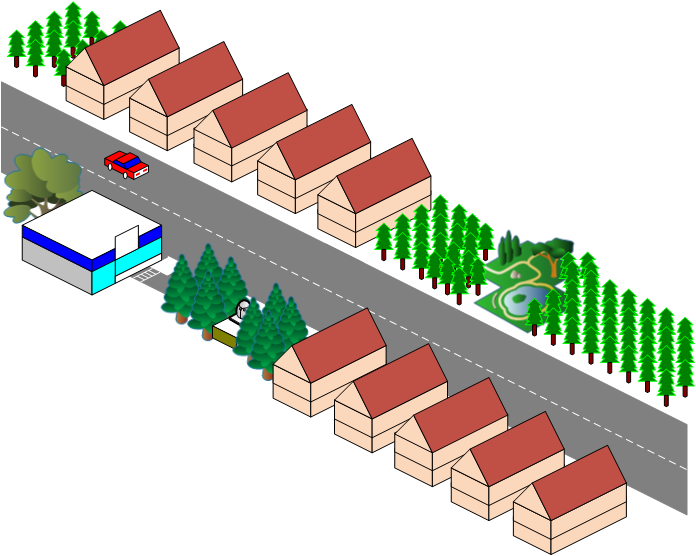
\includegraphics[scale=0.90]{../img/Dibujo1.png}
		\caption{Plano general de la urbanización}
	\end{figure}


\begin{landscape}
	\begin{figure}[H]
		\centering
		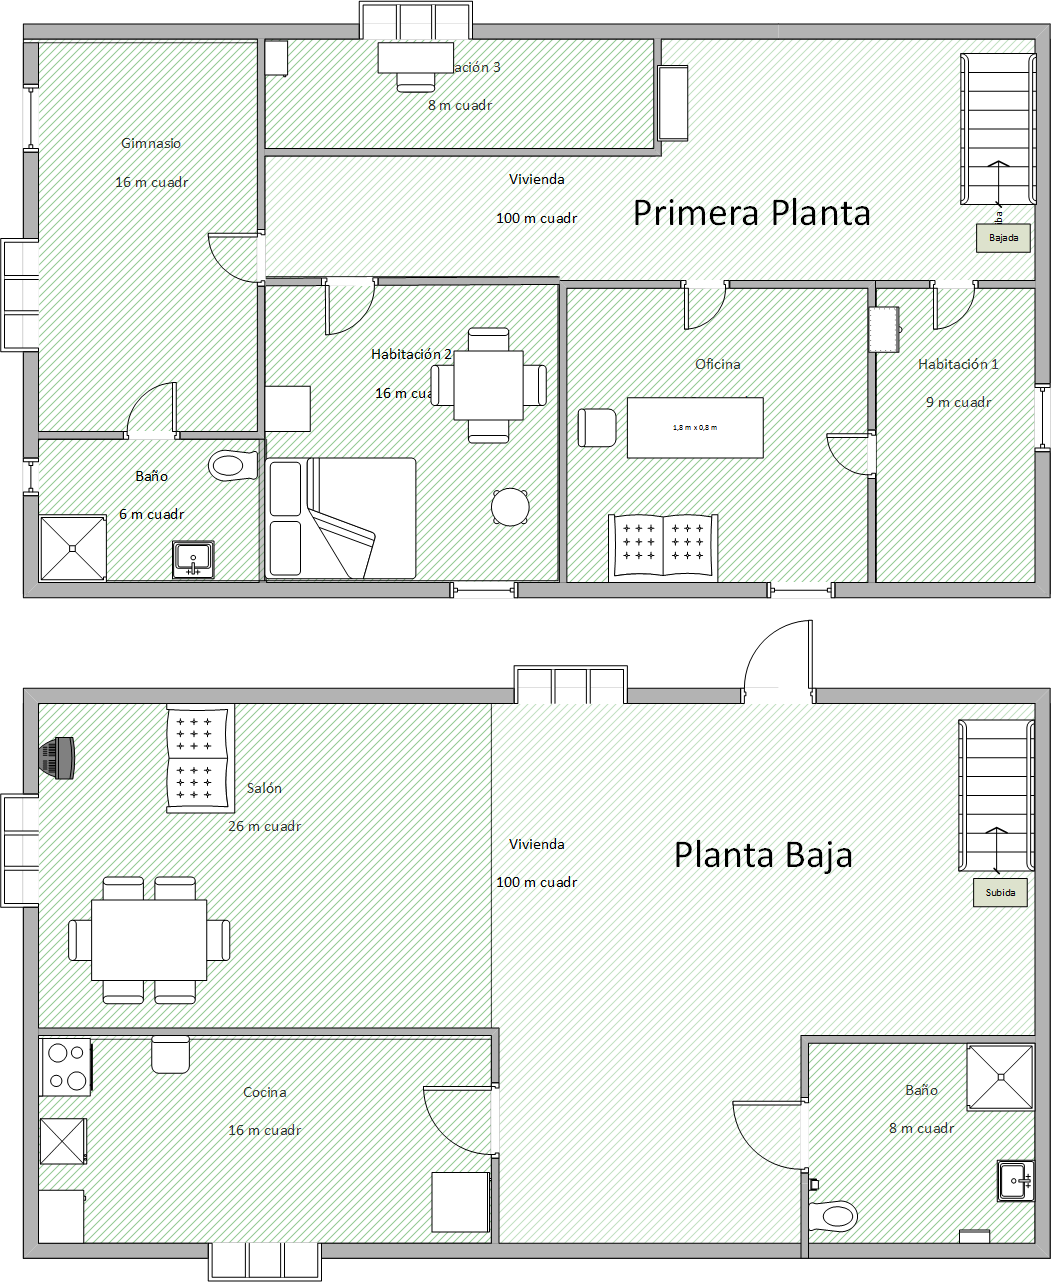
\includegraphics[scale=0.80]{../img/PlanoVivienda.png}
		\caption{Plano de la primera planta}
	\end{figure}
\end{landscape}

\begin{landscape}
	\begin{figure}[H]
		\centering
		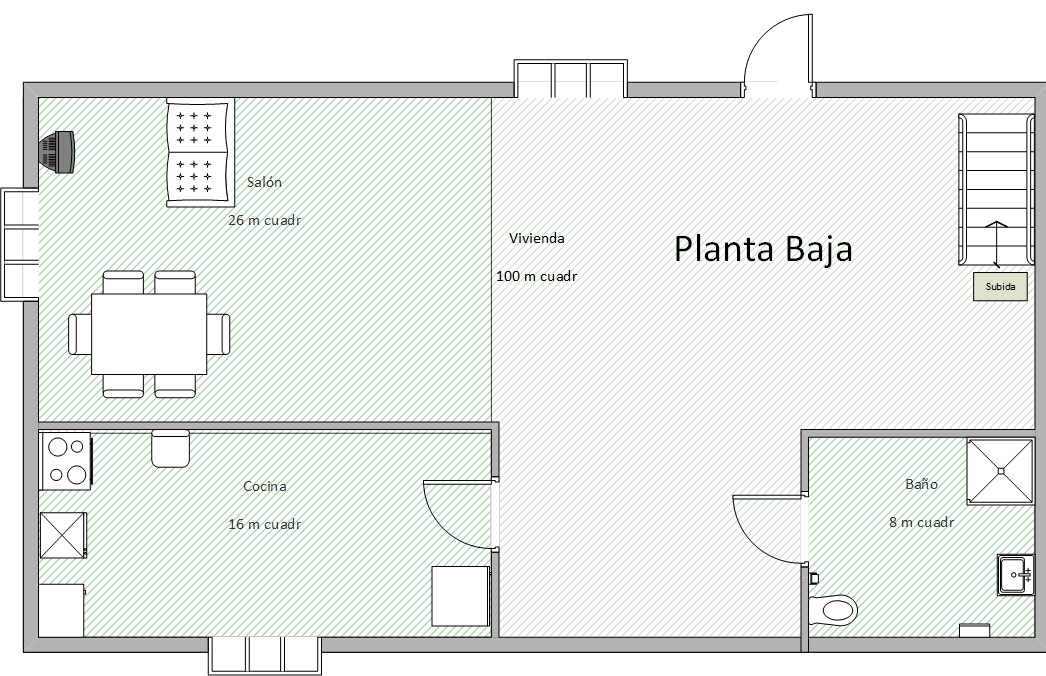
\includegraphics[scale=0.80]{../img/PlanoVivienda2.png}
		\caption{Plano de la segunda planta}
	\end{figure}
\end{landscape}

\begin{landscape}
	\begin{figure}[H]
		\centering
		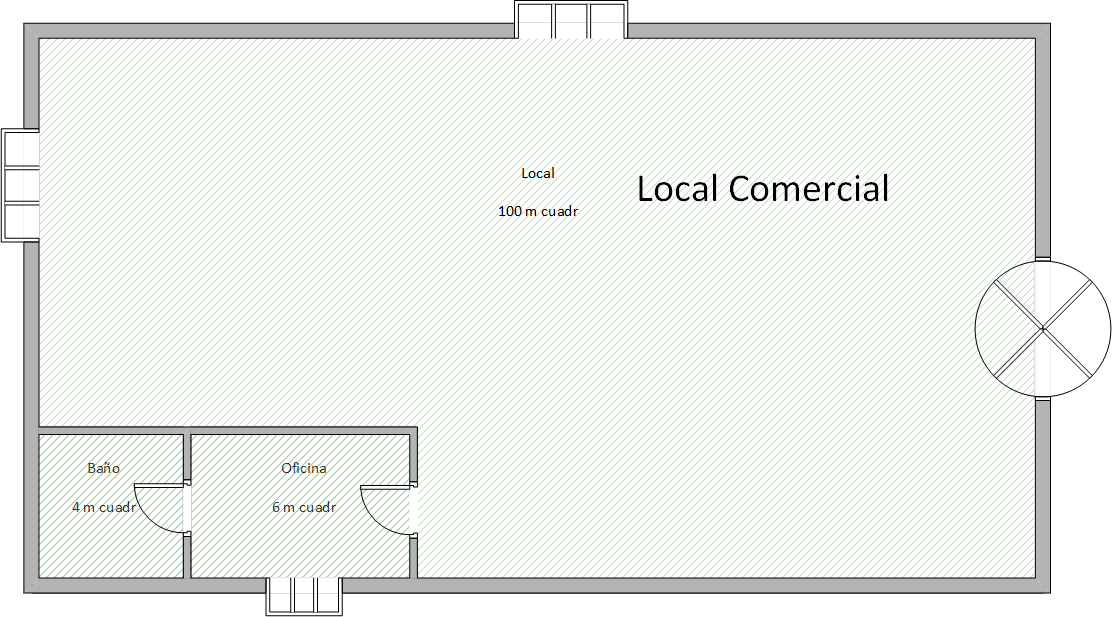
\includegraphics[scale=0.90]{../img/PlanoLocal.png}
		\caption{Plano del local comercial}
	\end{figure}
\end{landscape}

\begin{landscape}
	\begin{figure}[H]
		\centering
		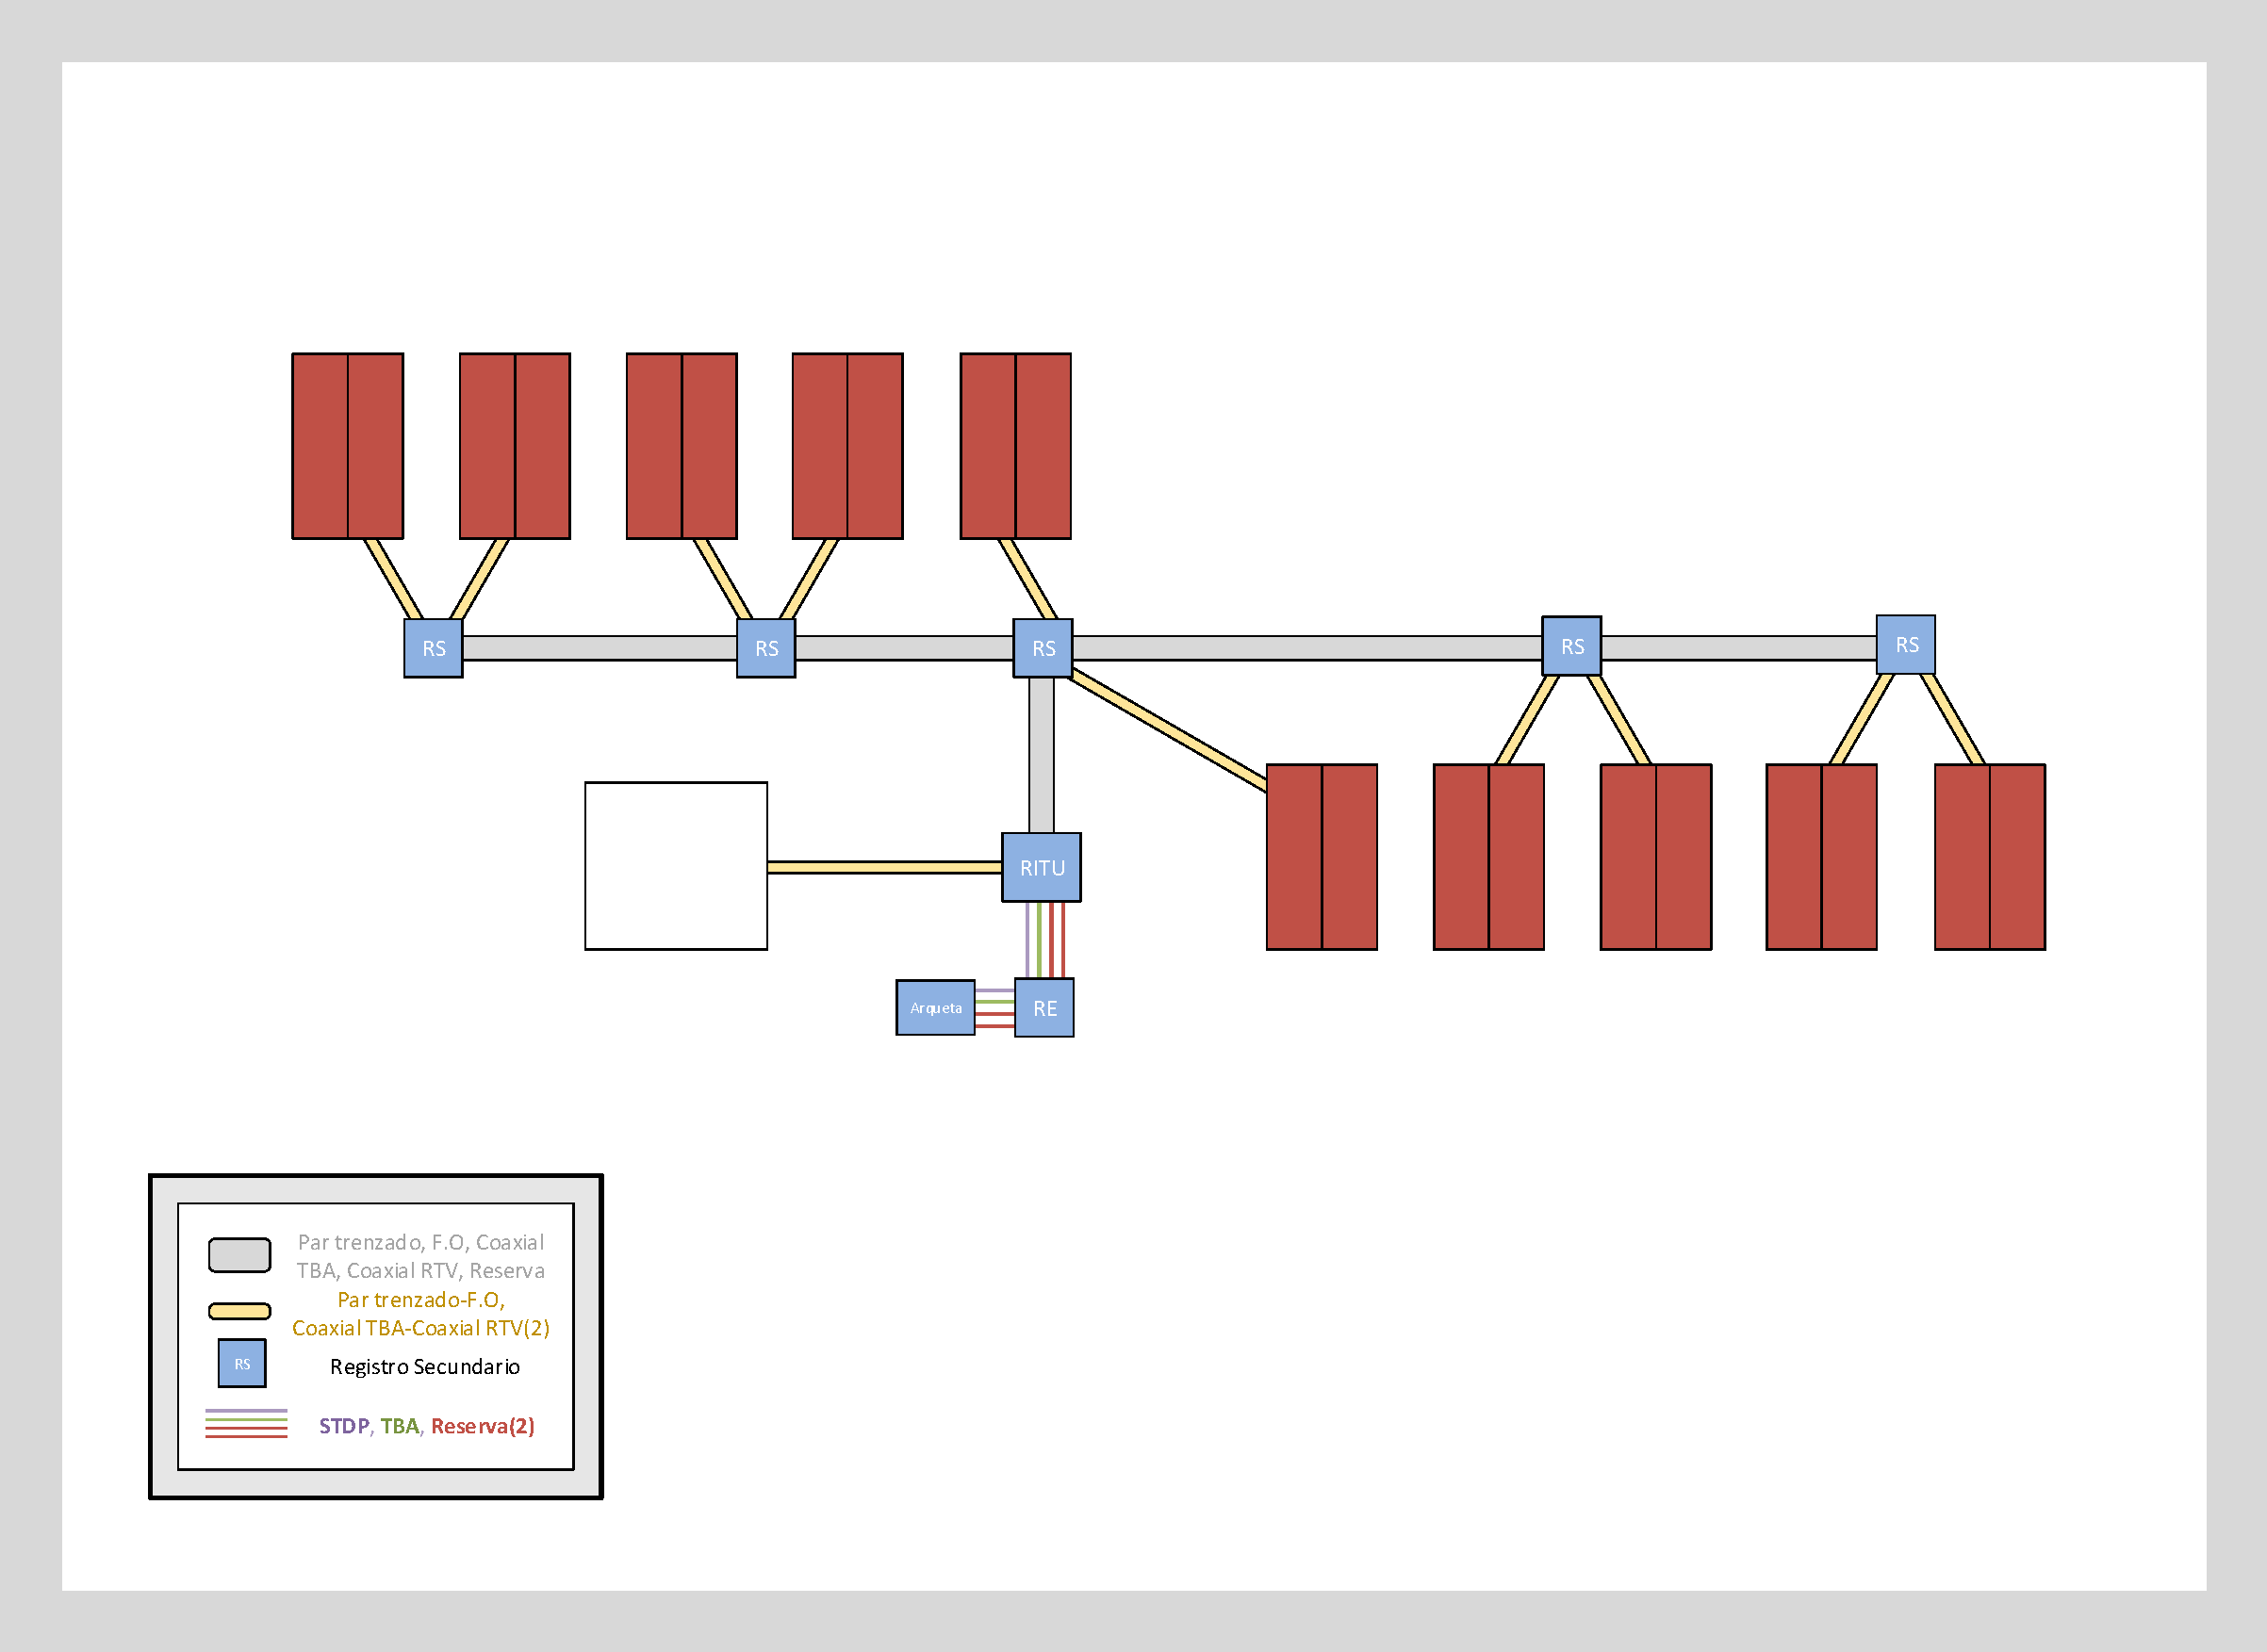
\includegraphics[scale=0.50]{../img/PLANOFINAL.pdf}
		\caption{Plano general de la instalación}
		\label{pla_general}
	\end{figure}
\end{landscape}

\begin{landscape}
	\begin{figure}[H]
		\centering
		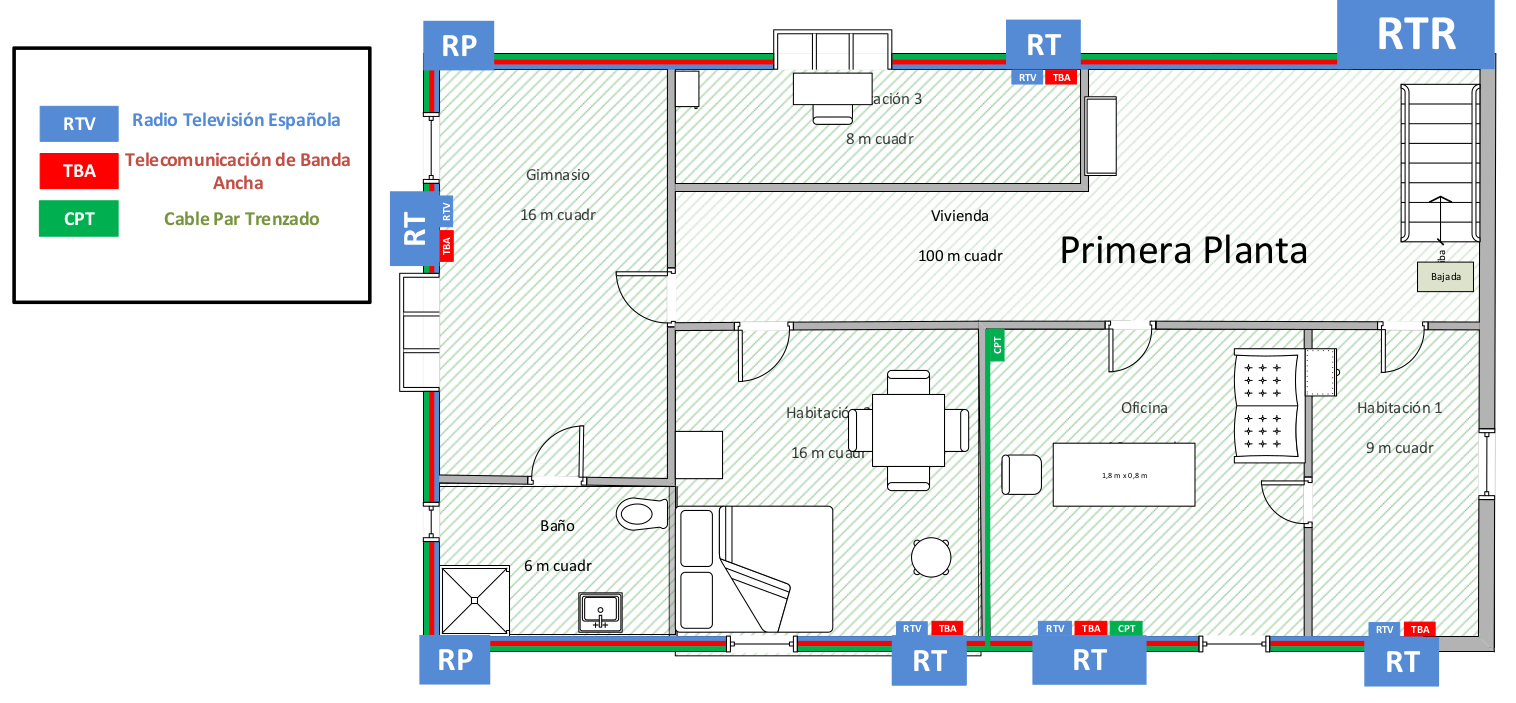
\includegraphics[scale=0.68]{../img/PlanoCableadoVivienda1.png}
		\caption{Plano de la primera planta con cableado}
	\end{figure}
\end{landscape}

\begin{landscape}
	\begin{figure}[H]
		\centering
		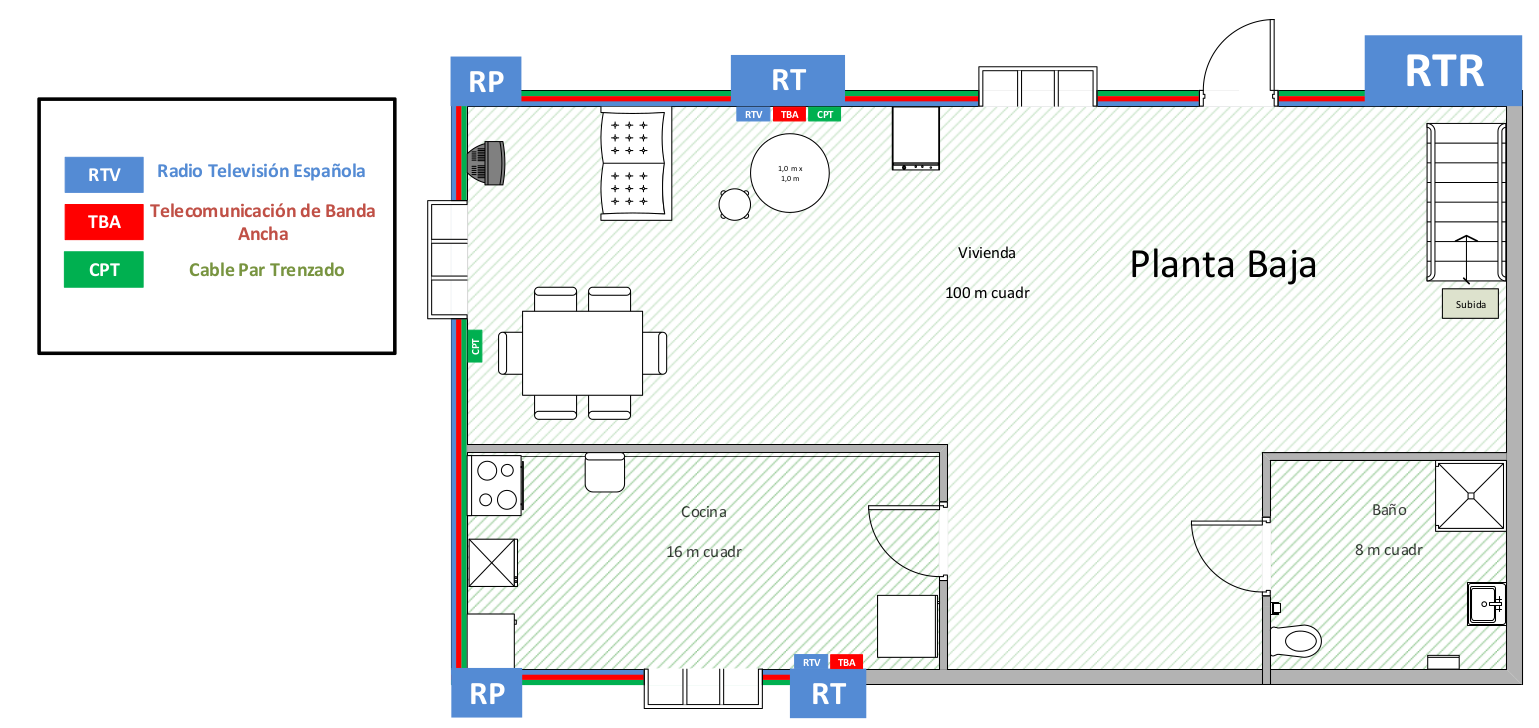
\includegraphics[scale=0.68]{../img/PlanoCableadoVivienda2.png}
		\caption{Plano de la segunda planta con cableado}
	\end{figure}
\end{landscape}

\chapter{PLIEGO DE CONDICIONES.}

\section{CONDICIONES PARTICULARES.}

\subsection{Radiodifusión sonora y televisión.}
\subsubsection{Condicionantes de acceso a los sistemas de captación.}
\subsubsection{Características de los sistemas de captación.}
\paragraph{Antenas.}
\paragraph{Elementos de sujeción de las antenas para televisión terrestre.}
\paragraph{Elementos de sujeción de las antenas para televisión por satélite}
\subsubsection{Características de los elementos activos.}
\subsubsection{Características de los elementos pasivos.}
\paragraph{Mezclador.}
\paragraph{Derivadores.}
\paragraph{Distribuidores.}
\paragraph{Cables.}
\paragraph{Punto de acceso al usuario.}
\paragraph{Bases de acceso de terminal.}

\subsection{Distribución de los servicios de telecomunicaciones de telefonía disponible al público (STDP) y de banda ancha (TBA).}
\subsubsection{Redes de cables de pares o pares trenzados.}
\paragraph{Características de los cables.}
\paragraph{Características de los elementos activos.}
\paragraph{Características de los elementos pasivos.}
\subsubsection{Redes de cables coaxiales.}
\paragraph{Características de los cables.}
\paragraph{Características de los elementos pasivos.}
\subsubsection{Redes de cables de fibra óptica.}
\paragraph{Características de los cables.}
\paragraph{Características de los elementos pasivos.}
\paragraph{Características de los empalmes de fibra en la instalación.}

\subsection{Infraestructura de hogar digital.}
\chapter{PRESUPUESTO.}


\end{document}
